\documentclass{article}
\usepackage[utf8]{inputenc}
\usepackage[english]{babel}

\usepackage{amsfonts}
\usepackage{amsthm}
\usepackage{amssymb}
\usepackage{amsmath}
\usepackage{tikz}
\usetikzlibrary{shapes.arrows,chains}

\theoremstyle{definition}
\newtheorem{definition}{Definition}[section]
\newtheorem{theorem}{Theorem}[section]
\newtheorem{example}{Example}[section]

\setlength{\parindent}{0pt}

\begin{document}

\tableofcontents

\section{Two problems}
Firstly we shall look at two problems which belong to the complexity class NP.

\subsection{Traveling Sales Person}
Consider a finite set $N$ of cities; $\{1, 2 \dots n\}$. The distance, or cost,
of traveling between cities $i$ and $j$ is given by $D(i,j)$ where $D$
is a symmetric matrix.

$$\forall\ i, j\quad D(i,J) \in \mathbb{N}\quad D(i,j) = D(j,i)$$

The problem is to find a path, or permutation, of
cities where each city appears exactly once in the path and the total
cost is minimised.

The brute force solution is to consider all paths, doing this would require
considering $!n$ paths.

\subsection{Boolean Formula Satisfiability}
A boolean formula consists of the logical binary operators $(\land, \lor, \neg)$
and a finite set of variables $X$ where each variable can be either true or false.
The problem consists of deciding if there exists a set of values for the variables $X$
which results in the boolean formula being true.

$$(x_1 \land x_2) \land \neg x_3$$

$$(x_1 \land x_2) \land \neg x_1$$

A brute force solution would be to consider all $2^{|X|}$ possible assignments.

The link between these two problems is the na\"ive brute force solution is not
tractable for large values of $n$.

\section{Turing Machines}
What do Turing machines do? Why are we looking at them?

Conceptually a turing machine is a \textit{tape} which is infinite in both directions,
the input is writen on this tape with the rest of the tape being blank. We have a head
which can read and write to the tape. The machine moves across the tape acording to
a transition function until it reaches a terminal state which produces a yes or no result.

\begin{center}
	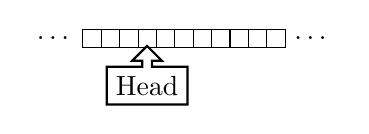
\begin{tikzpicture}[
	  start chain=1 going right,start chain=2 going below,node distance=-0.15mm
	]
		\node [on chain=1] at (-1.5,-.4) {\ldots};
		\foreach \x in {1,2,...,11} {\x, \node [draw,on chain=1] {}; }
		\node [
			name=k,
			arrow box,
			on chain=2,
			arrow box arrows={north:.25cm},
			draw=black,thick
			] at (-0.335,-1) {Head};
		\node [name=r,on chain=1] {\ldots};
	\end{tikzpicture}
\end{center}

\begin{definition}
	Formally a Turing machine consists of
	\begin{itemize}
		\item A \textit{tape alphabet} $\Gamma$ $\{a_1, a_2 \dots a_n, \beta\}$,
			where $a_i$ is a symbol, and $\beta$ is the blank or empty symbol.
		\item An \textit{input alphabet} $\Sigma$
			where $\Sigma \subset \Gamma \setminus \{\beta\}$.
		\item A set of states $Q$ $\{q_0, q_1 \dots q_m, q_y, q_n\}$ where $q_0$ is the
			initial state, $q_y$ is the terminal yes state, and $q_n$ is the terminal no state.
			$Q\prime = Q \setminus \{q_y,q_n\}$, i.e. the non-terminal states.
		\item A transition function $\delta$,
			where $\delta\ :\ (Q\prime \times \Gamma) \rightarrow
			(Q \times \Sigma \times \{L,S,R\})$.
			What this means is we look at a pair of a non-terminal state
			and a symbol from the alphabet;
			given this we enter a new state $q \in Q$,
			we write to the tape a symbol $a \in \Gamma$,
			and we stay or move the head left or right $(\{L,S,R\})$.
	\end{itemize}
\end{definition}

\begin{definition}
	Given an input $n$ and a Turing machine,
	$T(n)$ is the amount of times the transition function 
	$\delta$ must be applied to reach a terminal state.
\end{definition}

\subsection{Even or odd}
\begin{example}
	In this example we will present a turing machine to decide if a number is even.
	\begin{itemize}
		\item Input: a number $x \in \mathbb{Z}$ in unary form; i.e. $\{1 = X, 2 = XX\dots\}$,
			thus $\Sigma = \{X\}$.
		\item Output: yes iff $x$ is even, otherwise no. I.e. the turing machine will finish
			in state $q_y$ iff $x$ is even.
		\item Transition function $\delta$ is described as a matrix below with the states
			$Q\prime = \{q_0,q_1\}$ and $\Sigma = \{X,\beta\}$,
			output is $(Q \times \Sigma \times \{L,S,R\})$.
		\begin{center}
			\begin{tabular}{ c c c }
					 & $q_0$           & $q_1$           \\
				X    & ($q_1,\beta,R$) & ($q_0,\beta,R$) \\
			 $\beta$ & ($q_y,\beta,S$) & ($q_n,\beta,S$) \\
			\end{tabular}
		\end{center}
	\end{itemize}
	For this Turing machine $T(n) = n + 1$.
\end{example}

\subsection{Recognising Palindromes}

A palindrome is any word such that the reversed word is equal to the word itself,
consider the alphabet $\Gamma = \{a,b\}$, examples of palindromes would be $a, aa, aba$ etc.
Can we construct a Turing machine which recognises palindromes for the alphabet $\Gamma$?

We can, we simply move forward and backward checking each letter at opposite ends is the same,
until the entire word has been checked.
This means for palindromes $T(n)$ is equal to $n + (n - 1) \dots + 1$. Thus
$$T(n) = \frac{n^2 + n}{2}$$

However in non palindrome cases, say $aaa \dots ab$, then $T(n)$ is very small.

\section{$O, \Omega, \Theta$ Notation}

\begin{definition}
	$O(n)$
\end{definition}

\begin{definition}
	$\Omega(n)$
\end{definition}

\begin{definition}
	$\Theta(n)$
\end{definition}
Bit on worst case vs average vs best case

Note that for some $n$ $T(n)$ will be very small and for others it will be much larger,
usually this leads us to consider the complexity of the Turing machine to be 


\section{Complexity class P}
\begin{definition}
	\textit{Class P} is the class of problems for which there exists a Turing machine
	which can be computed in polynomial time.
\end{definition}

\section{Non-Deterministic Turing Machines}

\section{Complexity class NP}
\begin{definition}
	\textit{Class NP} is the class of problems 
\end{definition}

\begin{theorem}
	$P \subset NP$
\end{theorem}

\begin{theorem}
	Let $\mathcal{L} \in NP$ there exist a polynomial p(n) and TM
	for solving $\mathcal{L}$ with complexity $O(2^{p(n)})$.
\end{theorem}

\section{Polynomial transformations}
\begin{definition}
	Consider two languages $\mathcal{L_1} \subset A_1$ and $\mathcal{L_2} \subset A_2$,
	$\mathcal{L_1}$ is said to be \textit{polynomially transformable} to $\mathcal{L_2}$ if
	$$\exists\ f : A_1 \rightarrow A_2$$
	such that $f$ can be computed with polynomially complexity and $f$ preserves the language. I.e.
	$$\forall\ x \in A_1\ x \in \mathcal{L_1}\ \mathrm{iff}\ f(x)\in \mathcal{L_2}$$
\end{definition}

Practically $\mathcal{L_1} \propto \mathcal{L_2}$ means that
$\mathcal{L_2}$ is not harder than $\mathcal{L_1}$;
i.e. if $\mathcal{L_2} \in P$ then $\mathcal{L_1} \in P$.
Furthermore this relation is transitive.
$$
  \mathcal{L_1} \propto \mathcal{L_2},\ 
  \mathcal{L_2} \propto \mathcal{L_3},\Rightarrow
  \mathcal{L_1} \propto \mathcal{L_3}
$$

\section{Polynomial equivalence}
\begin{definition}
	If we have two languages such $\mathcal{L_1} \propto \mathcal{L_2}$ and
	$\mathcal{L_2} \propto \mathcal{L_1}$, then they are said to be \textit{polynomially equivalent}.
	Thus we have $\mathcal{L_1} \approx \mathcal{L_2}$.
\end{definition}

This is an equivalence as such it is transitive, symmetric, and reflexive;
as such $\forall\ \mathcal{R},\ \mathcal{S},\ \mathcal{T}$:
\begin{center}
	$\mathcal{R} \approx \mathcal{R}$\\
	if $\mathcal{R} \approx \mathcal{S}$ then $\mathcal{S} \approx \mathcal{R}$.\\
	$
		\mathcal{R} \approx \mathcal{S},\ 
		\mathcal{S} \approx \mathcal{T} \Rightarrow
		\mathcal{R} \approx \mathcal{T}
	$
\end{center}

%%TODO
In practise what this means is that we can see what problem a class is in if we can
polynomially translate it to another problem in a known class; for example:
$$
  \forall\ \mathcal{L_1} \in P\ 
  \forall\ \mathcal{L_2} \in P\ 
  \mathcal{L_1} \approx \mathcal{L_2}
$$

\section{NP-Complete problems}
\begin{definition}
	$\mathcal{L}$ is \textit{NP-Complete} if
	\begin{itemize}
		\item $\mathcal{L} \in NP$
		\item $\forall\ \mathcal{L\prime} \in NP\ \mathcal{L\prime} \propto \mathcal{L}$
	\end{itemize}
\end{definition}

What does this definition mean?
Any two NP-complete languages are polynomially equivalent.
Any NP-Complete problem is at least as hard as any other problem in NP.

\begin{theorem}
	Given two languages $\mathcal{S}, \mathcal{T} \in NP$,
	if $\mathcal{S} \in NPC$ and $\mathcal{S} \propto \mathcal{T}$ then
	$\mathcal{T} \in NPC$.
\end{theorem}

This theorem is rather useful for proving that a language is NP-Complete,
however it leaves us with the issue of proving a first language is NP-Complete.

\begin{definition}
	A boolean formula $F$ is in \textit{conjunctive normal form} if it is in the form
	\begin{equation}
	\begin{split}
		F &= f_1 \land f_2 \dots \land f_n \\
		f_i &= y_1 \lor y_2 \dots \lor y_m \\
		y_j &= x\ |\ \neg x
	\end{split}
	\end{equation}
\end{definition}

The following is in conjunctive normal form:
$$(x_1 \lor x_2) \land \neg x_3$$
The following is not in conjunctive normal form;
however it is in \textit{disjunctive normal form}
$$(x_1 \lor x_2) \lor \neg x_3$$
This is because there is the negation on the left hand side of the logical or.

\begin{definition}
	Given an undirected graph $\mathcal{G}$ which is a pair of vertices and edges $(V,E)$,
	a subset of vertices $S \subset V$ is a \textit{clique} iff
	$$\forall\ x, y \in S\ \exists\ \textrm{an edge}\ (x,y) \in E$$
\end{definition}

\begin{definition}
	If $S$ is a clique in $\mathcal{G}$ and $|S| = q$ then $S$ is called a \textit{$q$-clique}.
\end{definition}

An obvious consequence of this definition is that for any edge $(x,y)$ there is a 2-clique.

\begin{definition}
	The \textit{$q$-clique problem} is finding if there exists a $q$-clique in a given graph
	$\mathcal{G}$ where $q \in \mathbb{N}$.
\end{definition}

\section{Cook’s Theorem}


\section{Structure of the class NP}
\subsection{Structure of the class NP}
\subsection{Complements to languages}
\subsection{Class co-NP}
\subsection{Some famous candidates for problems in NPI}
\subsubsection{Graph Isomorphism}
\subsubsection{Linear Programming}
\subsection{Search problems}
\subsection{Turing transformation}
\subsubsection{Turing transformation: informal definition}
\subsubsection{Oracle Turing Machine}
\subsubsection{Turing transformation: definition}
\subsection{NP-hard problems}
\subsection{NP-hard problems}
\subsection{NP-hard problems}



\section{Approximate Algorithms}
Many problems in NP-hard are problems for which we need a polynomial algorithm;
thus we are left with few, but not none, options.
It may be the case that we can find an algorithm for our relevant cases.
Alternatively we may need to solve the problem for the input
data of a relatively small size, so that even an exponential-time algorithm is acceptable.
Finally, we can try to solve the problem approximately;
i.e. solve the problem as close to optimally as possible but accept some degree of error
or incorrectness.
This last approach is suitable for optimization search problems.

Examples of optimization search problems.
\begin{itemize}
    \item Travelling Salesperson (find the smallest tour)
    \item Find the largest clique in a graph
    \item Vertex Covering (find the smallest covering)
\end{itemize}

\subsection{Ratio bound and relative error}
For approximation algorithms we need an \textit{objective function}
which will allow us to measure the difference of the approximate and optimal algorithms.
For example in the traveling sales person problem,
the objective function is the length of the tour produced by the algorithm.
We want to determine how "close" our approximate algorithm is to the
optimal one.  We define "closeness" as \textit{ratio bound and relative error bound}.

We will assume that the objective function is always positive.

Let $C$ denote the value of the objective function at our approximate solution,
and $C\prime$ at an optimal solution.

\subsubsection{Ratio Bound}
\begin{definition}
    An approximation algorithm has \textit{ratio bound $\rho(n)$}
    if for any input of the size $n$ the value $C$ of the objective function
    at the approximate solution satisfies the inequality
    $$
    max(C/C\prime, C\prime/C) \leq \rho(n)
    $$
\end{definition}

Observe that
$$ 0 < C \leq C\prime $$
thus for maximization problems
$$ max(C/C\prime, C\prime/C) = C\prime/C $$
and for minimization problems
$$ max(C/C\prime, C\prime/C) = C/C\prime $$

Firstly observe that $\rho(n) \geq 1$,
and secondly that when $\rho(n) = 1$ we have an optimal solution.
By definition a large ratio bound (might) means that the approximate
solution is much worse than an optimal one.
This is an issue of trading speed for correctness.

\subsubsection{Relative Error Bound}
\begin{definition}
    For $C, C\prime$ and $n$  the \textit{relative error bound $\epsilon(n)$} is defined as
    $$\frac{abs(C - C\prime)}{C\prime} \leq \epsilon(n)$$
\end{definition}

Observe that $\rho(n) - 1 \leq abs(C\prime - C)/C\prime$,
i.e., $\rho(n) - 1$ is a relative error bound.

\subsection{Approximation algorithm for Vertex Covering}


\subsection{Approximation algorithm for Travelling Salesman with triangle inequality}
Given a connected graph $\mathcal{G}\ (V,E)$,
\begin{enumerate}
    \item
        Choose a vertex $v \in V$, to serve as the root of a tree.
        Build a spanning tree $T$ beginning at $v$;
        note that this can be done in polynomial time using Prim's or Kruskal's algorithm.
    \item
        Perform a pre-order walk on the tree $T$ returning the list of nodes as a tour.
\end{enumerate}

We can now propose three properties of this algorithm
\begin{enumerate}
    \item It is correct
    \item It has polynomial complexity
    \item It has a ratio bound $\rho(n) = 2$
\end{enumerate}

\end{document}
